\begin{figure}[h]
	\centering
	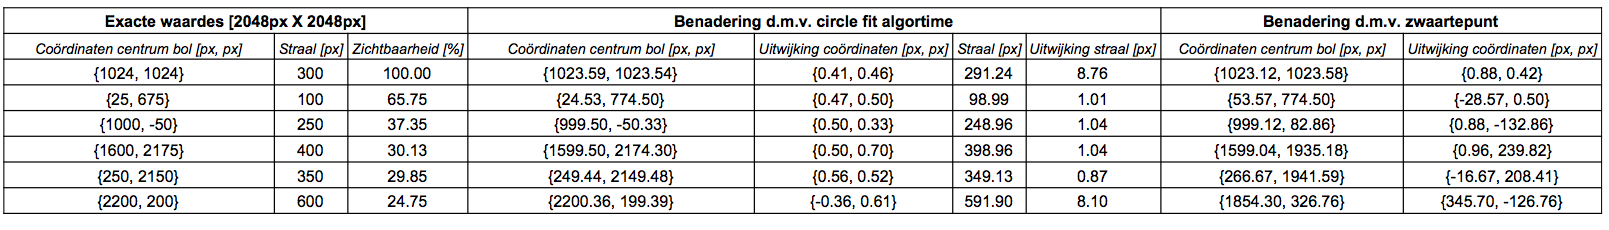
\includegraphics[width=0.9\textwidth]{TestData.png}
	\caption{Deze testdata van de \textit{ImageCalculation} geeft de verschillen weer tussen beide algoritmes die gebruikt worden om de afstand van de bol te berekenen. Het is duidelijk dat het circle-fit algoritme beduidend minder afwijkt van de correcte waardes dan het algoritme op basis van het zwaartepunt (cog). Hoe minder de bol zichtbaar is, hoe groter de afwijking.}
\end{figure}